\documentclass[presentation]{beamer}

\usepackage{tikz}
\usetikzlibrary{positioning,calc}
\usetikzlibrary{shapes.geometric}
\usetikzlibrary{backgrounds}% only to show the bounding box
\usetikzlibrary{shapes,arrows}
\usepackage{pgfplots}
\usepackage{pgfplotstable}
\usetikzlibrary{pgfplots.groupplots}
\pgfplotsset{compat=1.12}
\usepackage{appendixnumberbeamer}
\usepackage{amsmath}
\date{20th May 2016}
\usetheme{firedrake}

\pgfplotscreateplotcyclelist{decent cycle}{%
  {blue, mark=*, mark options={fill=blue},
    mark size=2pt},
  {cyan, mark=square*, mark options={fill=cyan},
    mark size=2pt},
  {magenta, mark=triangle*, mark options={fill=magenta},
    mark size=3pt},
  {blue, mark=*, mark options={fill=blue},
    mark size=2pt},
  {cyan, mark=square*, mark options={fill=cyan},
    mark size=2pt},
  {magenta, mark=triangle*, mark options={fill=magenta},
    mark size=3pt},
}

\pgfplotsset{
  decent/.style={
    cycle list name=decent cycle,
  }
}
\renewcommand{\vec}[1]{\ensuremath{\boldsymbol{#1}}}
\newcommand{\ddt}[1]{\frac{\partial #1}{\partial t}}
\newcommand{\zhat}{\hat{\vec{z}}}
\newcommand{\W}{\ensuremath{\mathbb{W}}}

\DeclareMathOperator{\grad}{grad}
\let\div\relax
\DeclareMathOperator{\div}{div}
\DeclareMathOperator{\curl}{curl}
\newcommand{\vsubset}[1]{\rotatebox[origin=c]{90}{\ensuremath{\subset}}}
\author{Lawrence Mitchell\inst{1} \and Eike M\"uller\inst{2}}
\institute{\inst{1}Departments of Computing and Mathematics, Imperial College London
  \and
  \inst{2}Department of Mathematical Sciences, University of Bath}
\title{Multigrid for numerical weather prediction}

\graphicspath{{./\jobname.figures/}}

\newcommand{\arxivlink}[2]{%
  \href{http://www.arxiv.org/abs/#1}%
  {{\small\texttt{arXiv:\,#1\,[#2]}}}%
}
\usepackage[url=false,
            doi=true,
            isbn=false,
            style=authoryear,
            firstinits=true,
            uniquename=init,
            backend=biber]{biblatex}

\setbeamertemplate{bibliography item}{}
\renewcommand{\bibfont}{\footnotesize}
\addbibresource{references.bib}

\setlength{\bibitemsep}{1ex}

\renewbibmacro{in:}{}
\DeclareFieldFormat[article]{volume}{\textbf{#1}}
\DeclareFieldFormat{doi}{%
  doi\addcolon%
  {\scriptsize\ifhyperref{\href{http://dx.doi.org/#1}{\nolinkurl{#1}}}
    {\nolinkurl{#1}}}}
\AtEveryBibitem{%
\clearfield{pages}%
\clearfield{issue}%
\clearfield{number}%
}

\usepackage{minted}

\begin{document}
% \begin{abstract}
%   In recent years, finite element methods have gained popularity in the
%   numerical weather prediction community due to their ability to deal
%   with non-orthogonal meshes and high order discretisations.  Compatible
%   (or mimetic) spaces offer some appealing features for models such as
%   stable discretisations of pressure gradients and geostrophic balance.
%   However, they present challenges in solving the elliptic system
%   resulting from implicit timestepping schemes.  The high aspect ratio
%   domains typical in these problems require us to treat the "vertical"
%   direction specially when designing a solver if we want to achieve
%   mesh-independent iteration counts.

%   In this talk I will discuss work in Firedrake on developing custom
%   geometric multigrid solvers for these problems and present an analysis
%   of the resulting performance, solving problems with up to two billion
%   degrees of freedom.
% \end{abstract}
\maketitle

\section{Introduction}

\begin{frame}
  \frametitle{Motivation}
  Weather forecasting centres moving from orthogonal
  lat-lon to non-orthogonal meshes (e.g.~cubed sphere, or icosahedral
  sphere).
  \begin{center}
    \begin{tikzpicture}
      \node (A) {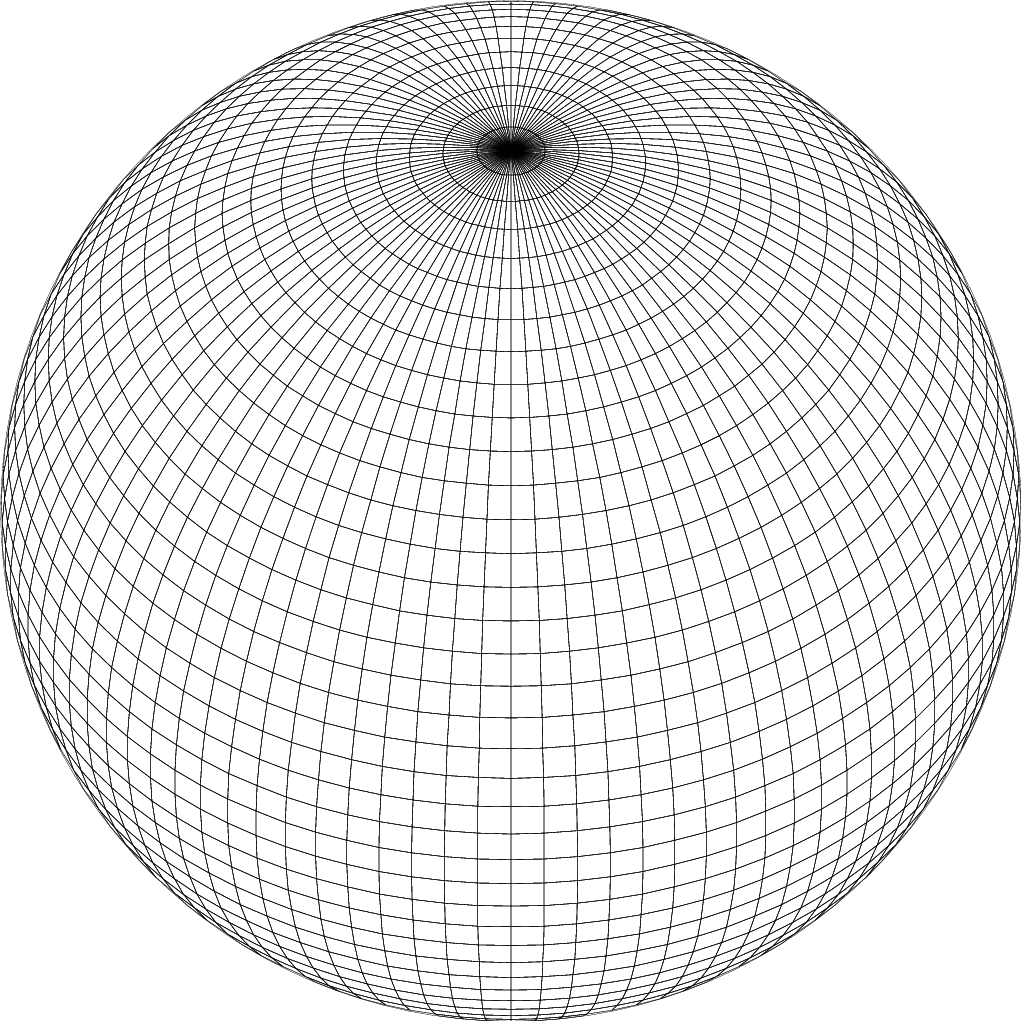
\includegraphics[width=2cm]{sphere-latlon}}; \node
      (B) [right=of A] {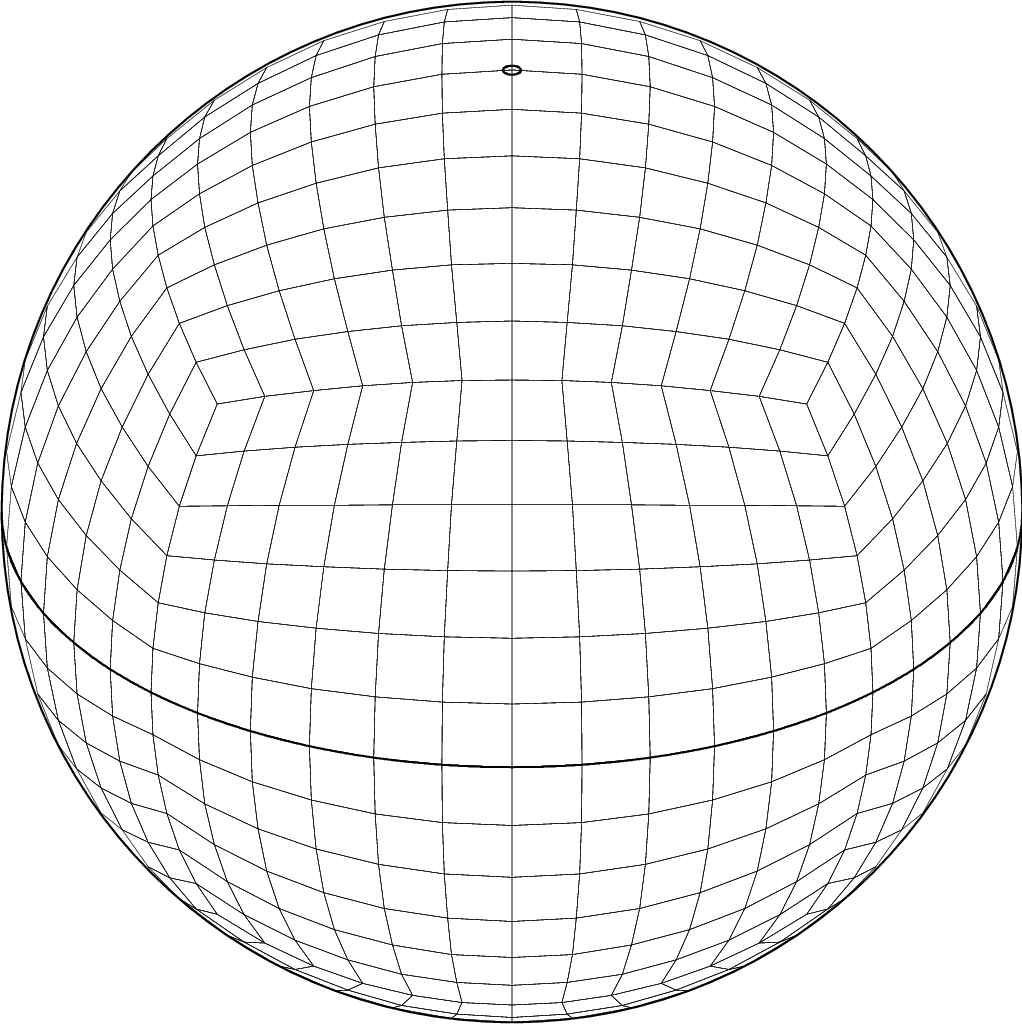
\includegraphics[width=2cm]{sphere-cubed}};
      \draw[-latex, very thick] (A)--(B);
    \end{tikzpicture}
  \end{center}
  Can no longer use traditional staggered finite differences.

  \emph{Compatible finite elements} (FEEC) a plausible
  solution \parencite{Cotter:2012a}.
\end{frame}

\begin{frame}
  \frametitle{Compatible FE}
  Choose discrete spaces that match the properties of the
  continuous equations.

  \begin{equation*}
    \begin{matrix}
      H^1 & & H(\curl) & & H(\div) & & L^2\\
      \vsubset{} & & \vsubset{} & & \vsubset{} & & \vsubset{} \\
      \W_0 & \stackrel{\grad}{\longrightarrow} &
      \W_1 & \stackrel{\curl}{\longrightarrow} &
      \W_2 & \stackrel{\div}{\longrightarrow} &
      \W_3
    \end{matrix}
  \end{equation*}

  \begin{block}{Tensor product spaces on wedges}
    \begin{center}
      \begin{tikzpicture}[scale=0.25]
        \node[thick, isosceles triangle, isosceles triangle apex
        angle=60, draw] (A) {};

        \node (B) [right=0.05cm of A] {$\otimes$};

        \node (C) [right=0.05cm of B, thick, rectangle, minimum
        width=0pt, inner sep=0pt, draw, minimum height=0.5cm] {};

        \draw[-latex, very thick] (C)++(0.5cm,0) -- +(2cm, 0);
        \begin{scope}[shift={($(C) + (3cm, -2cm)$)}]
          \draw[thick] (0,0) rectangle (4,4); \draw[thick] (0,0) --
          (1,1); \draw[thick] (4,0) -- (1,1); \draw[thick] (0,4) --
          (1,5); \draw[thick] (4,4) -- (1,5); \draw[thick] (1,1) --
          (1,5);
        \end{scope}
      \end{tikzpicture}
    \end{center}
  \end{block}
\end{frame}

\begin{frame}
  \frametitle{Computational challenges}
  Dynamical core needs to handle fast acoustic waves
  implicitly.

  Need a solver that is \emph{scalable} and \emph{fast}.

  $5$km horizontal, 100 vertical layers, around $2 \cdot 10^9$ dofs.

  Large aspect ratio of the domain is challenging for black box
  solvers.
\end{frame}

\section{Formulation}

\begin{frame}
  \frametitle{Linearised gravity wave}
  Linear system for velocity $\vec{v}$, pressure $p$, and buoyancy $b$.
\vspace{2em}

  \begin{columns}
    \begin{column}{0.4\textwidth}
      \begin{align*}
        \ddt{\vec{v}} &= \nabla p + b \zhat, \\
        \ddt{p} &= -c^2 \nabla\cdot \vec{v}, \\
        \ddt{b} &= -N^2\vec{v}\cdot\zhat.\\
      \end{align*}
    \end{column}
    \begin{column}{0.6\textwidth}
      Enforce $\vec{v}\cdot \hat{\vec{n}} = 0$ at top and bottom.\\
      $R\approx 6000\textsf{km}$, $H\approx 80\textsf{km}$. \\
      \begin{center}
        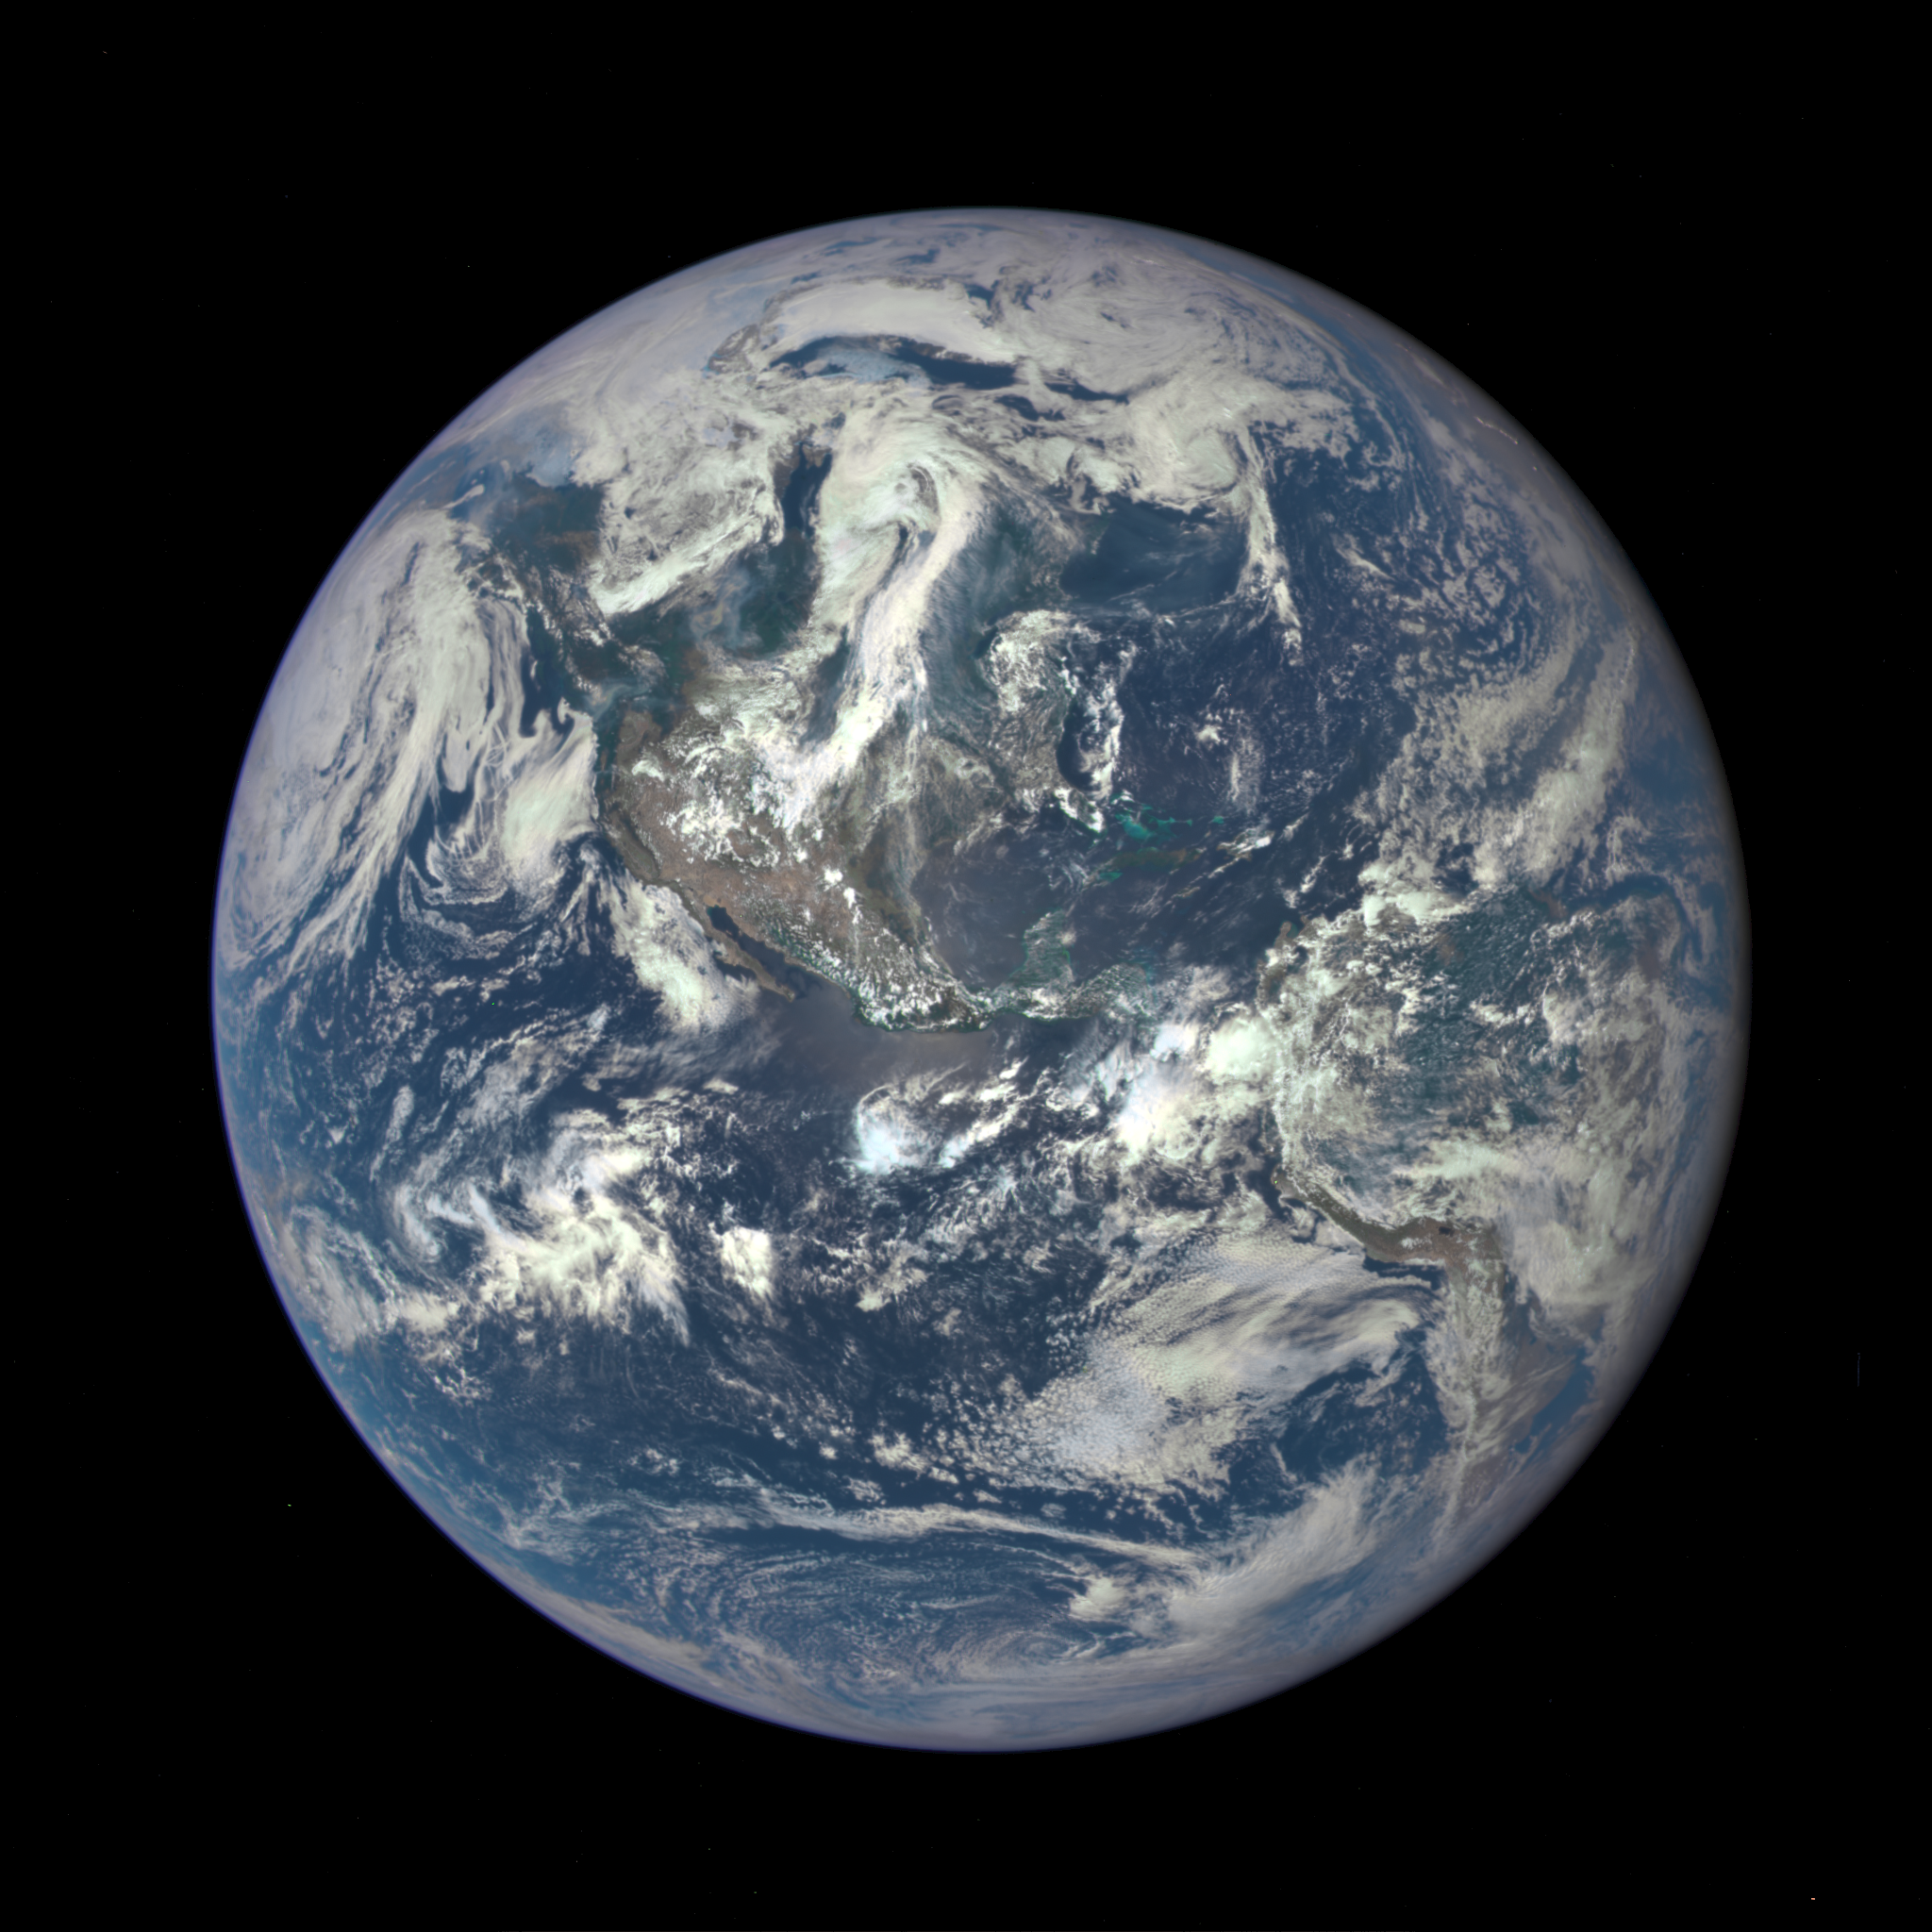
\includegraphics[width=3cm]{earth}
      \end{center}
    \end{column}
  \end{columns}
\end{frame}

\begin{frame}
  \frametitle{Discretised system}
  After discretising in space and time we obtain a linear operator for
  $\vec{v} \in H(\div)$, $p \in L^2$, $b$ scalar, collocated with
  vertical part of $\vec{v}$ space.
\begin{equation*}
\begin{pmatrix}
  M_v &
    -\frac{\Delta t}{2}D^T &
    -\frac{\Delta t}{2}Q\\[1ex]
  \frac{\Delta t}{2}c^2D & M_p & 0\\[1ex]
  \frac{\Delta t}{2}N^2Q^T & 0 & M_b
\end{pmatrix}
\end{equation*}
\end{frame}

\begin{frame}
  \frametitle{Preconditioning}
  Eliminate buoyancy pointwise in preconditioner.  Exact for spherical earth,
  approximate when mountainous.

  Obtain a velocity-pressure system
\begin{equation*}
\begin{pmatrix}
  M_v & -\frac{\Delta t}{2}D^T\\
  \frac{\Delta t}{2}c^2D & M_p\\
\end{pmatrix}
\end{equation*}

\end{frame}

\begin{frame}[t]
  \frametitle{Options}
  \begin{columns}
    \begin{column}{0.52\textwidth}
      \begin{block}{Block diagonal}
        Using the appropriate function space inner products \parencite{Mardal:2011,Kirby:2010}
        \begin{equation*}
          \begin{pmatrix}
            (I - \grad \div)^{-1} & 0 \\
            0 & I\\
          \end{pmatrix}
        \end{equation*}
      \end{block}
      \begin{itemize}
      \item All operators sparse
      \item $H(\div)$ multigrid \parencite{Arnold:2000} is challenging
      \end{itemize}
    \end{column}
    \begin{column}{0.52\textwidth}
      \begin{block}{Schur complement}
        Block elimination and back substitution
        \begin{equation*}
          \begin{pmatrix}
            M_v^{-1} & 0 \\
            0 & (M_p + \omega_c^2 D M_v^{-1} D^T)^{-1}\\
          \end{pmatrix}
        \end{equation*}
      \end{block}
      \begin{itemize}
      \item $S = M_p +  \omega_c^2 D M_v^{-1} D^T$ is \emph{dense}, but elliptic
      \item Can use similar methods as a \emph{distributive} smoother.
      \end{itemize}
    \end{column}
  \end{columns}
\end{frame}

\begin{frame}[allowframebreaks]
  \frametitle{Approximating $S$}
  \begin{itemize}
  \item Strong coupling in vertical direction, need to treat this
    exactly.
  \item Use a multigrid cycle with horizontal coarsening and
    vertical line relaxation.
  \item Exploit tensor-product structure to split horizontal and
    vertical components.
  \end{itemize}
  \framebreak

  \begin{itemize}
  \item Split horizontal and vertical $M_v^{-1} =
    (M_v^h)^{-1}\oplus (M_v^z)^{-1}$ (also $D
    = D^h \oplus D^z$)
  \item Diagonal approximation $M_v^{-1} \approx M_{v,\text{inv}} = \delta_{ij} / (M_v)_{ii}$
  \item Ignore horizontal coupling, error $\mathcal{O}((\Delta z/
    \Delta x)^2)$
  \end{itemize}
  \begin{block}{Final approximation}
    \begin{equation*}
      \tilde{S} = M_p + \omega_c^2 \text{bdiag}\big[D^h M_{v,\text{inv}}^h
      (D^h)^T\big] \oplus \frac{\omega_c^2}{1 + \omega_N^2} D^z
      M_{v,\text{inv}}^z (D^z)^T
    \end{equation*}
  \end{block}
\end{frame}

\begin{frame}[fragile, allowframebreaks]
  \frametitle{Implementation}
  Multigrid V-cycle using exact inverse of $\tilde{S}$ as smoother.
  Utilise column innermost numbering to perform fast banded matrix
  inverse
  \begin{center}
    \begin{tikzpicture}
      \node (A) {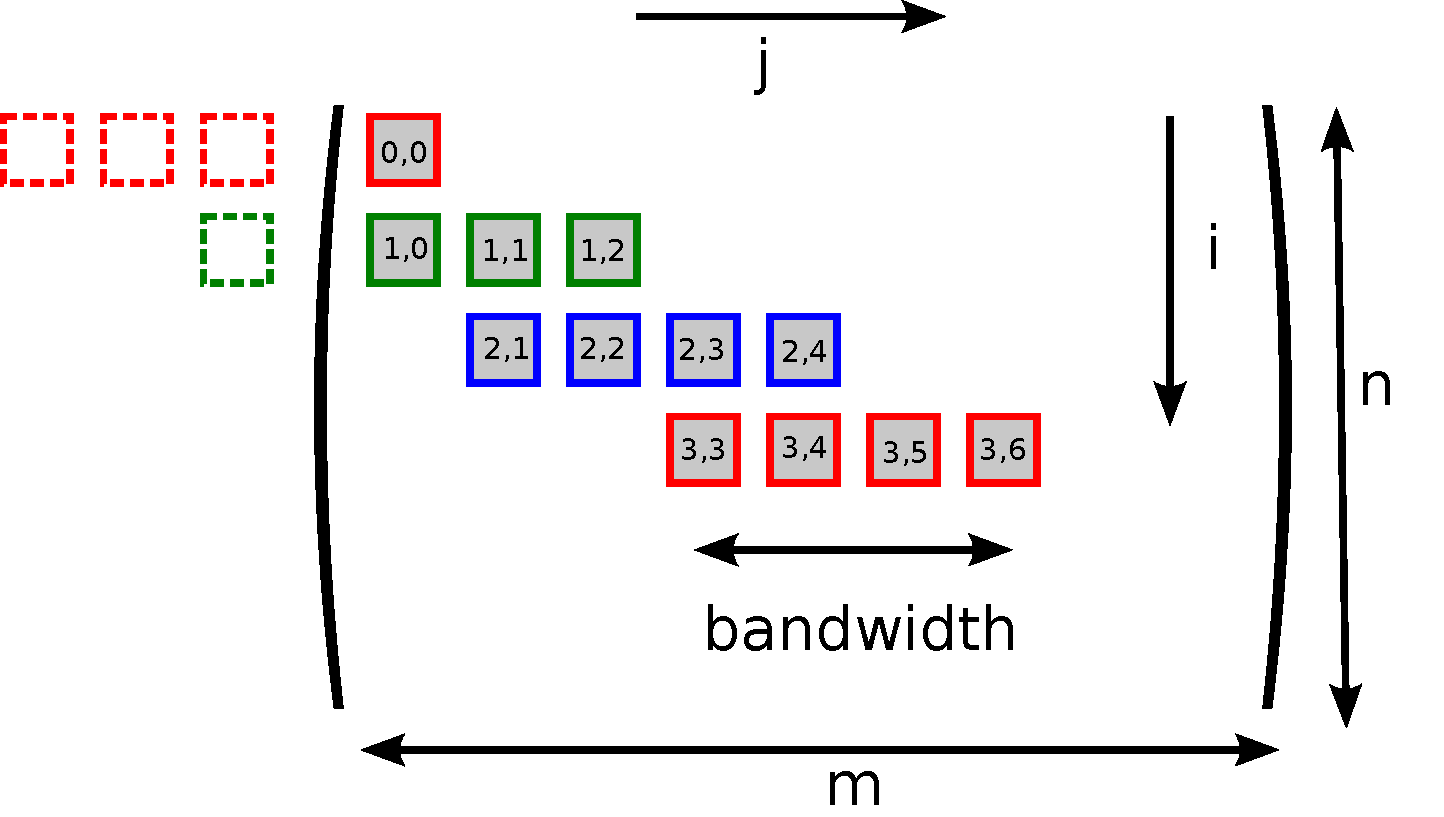
\includegraphics[height=2.5cm]{bandedmatrix}};
      \node (C) [right=of A.north east, anchor=north west] {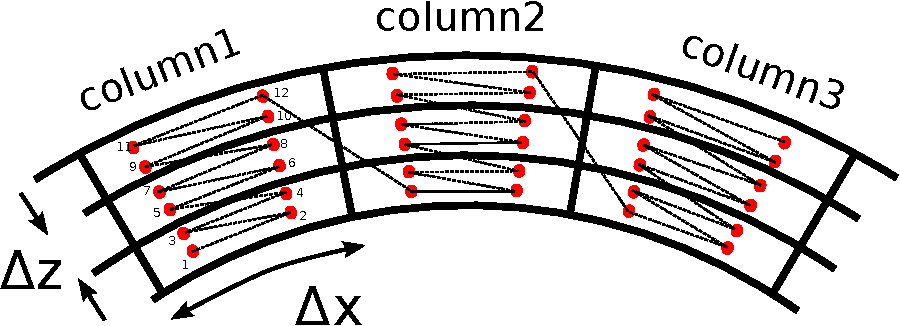
\includegraphics[width=3.5cm]{columndofs}};
      \node (B) [below=0.1cm of C] {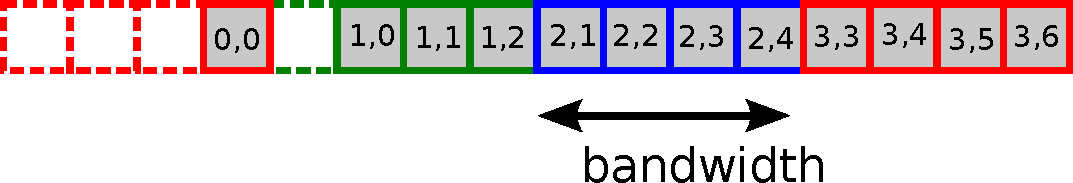
\includegraphics[height=0.6cm]{linearstorage}};
      \node (D) [above=0.1cm of A.north east, anchor=south] {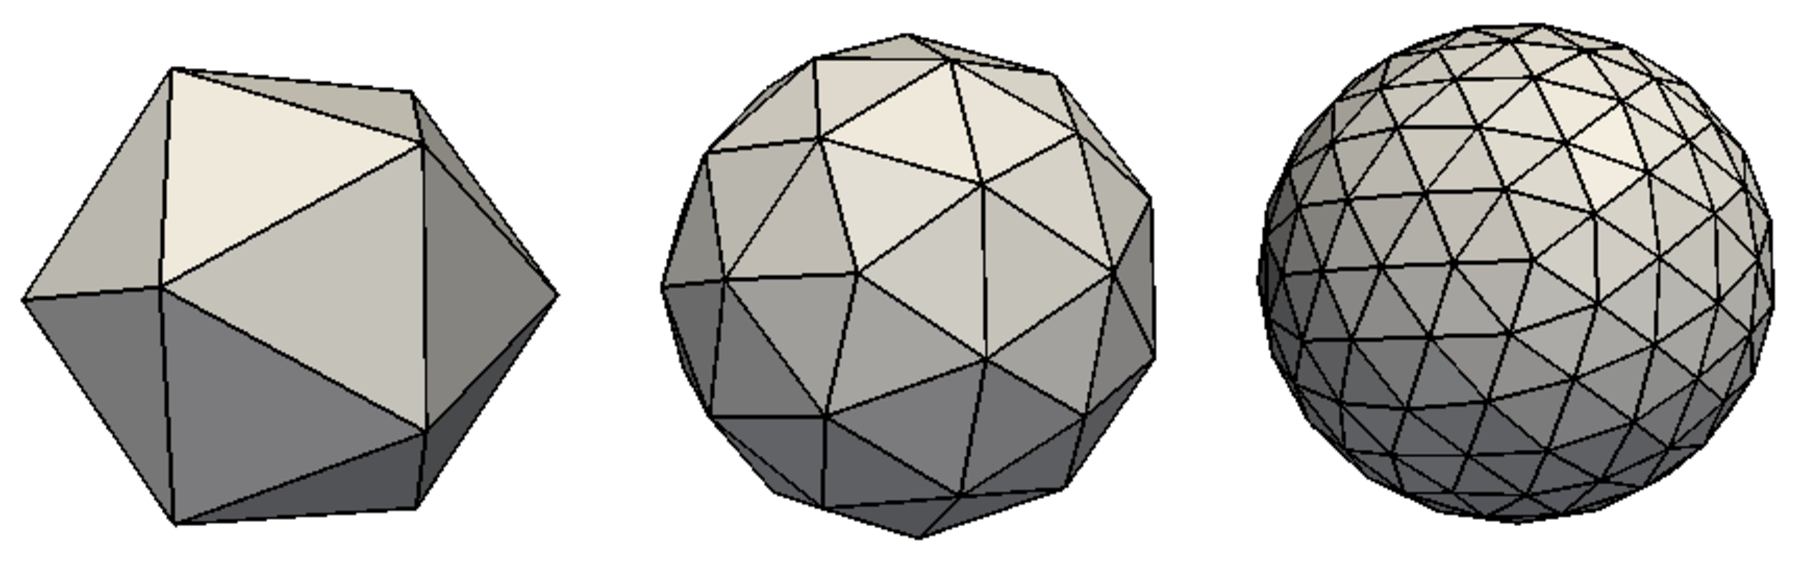
\includegraphics[width=5cm]{MeshHierarchy}};
    \end{tikzpicture}
  \end{center}

\framebreak

Banded matrix algebra implemented as short PyOP2 kernels (Firedrake's
\emph{escape hatch})

\begin{minted}[fontsize=\tiny]{python}
# C-kernel code for Matrix-vector product v = A.u in one vertical column
kernel_code = '''void ax(double **A, double **u, double **v) {
  for (int i = 0; i < n_row; ++i) {
    v[0][i] = 0.0;
    int j_m = (int)ceil((alpha*i - gamma_p)/beta);
    int j_p = (int)floor((alpha*i + gamma_m)/beta);
    for (int j = std::max(0, j_m); j < std::min(n_col, j_p+1); ++j)
      v[0][i] += A[0][bandwidth*i + (j - j_m)] * u[j];
  }'''
# Execute PyOP2 kernel over grid
kernel = op2.Kernel(kernel_code, 'ax', cpp=True)
op2.par_loop(kernel, hostmesh.cell_set,
             A(op2.READ, Vcell.cell_node_map()),
             u.dat(op2.READ, u.cell_node_map()),
             v.dat(op2.WRITE, u.cell_node_map()))
\end{minted}

\framebreak

\begin{itemize}
\item Use PETSc to solve block system with fieldsplit preconditioner.
\item Preconditioner for $S$ a \verb|PCSHELL| implementing custom
  multigrid.
\item Allows comparison with purely algebraic approach.
\end{itemize}
\end{frame}

\section{Results}

\begin{frame}
  \frametitle{Compare three solvers to invert $S$}
  GMRES(30) + full schur complement factorisation tolerance $10^{-5}$.

  \begin{block}{Single level}
    Two smoother iterations just on fine level (standard approach in
    Met Office Unified Model).
  \end{block}

  \begin{block}{Custom MG}
    Bespoke multigrid, 5 levels.  1 smoother sweep per level.  2 smoother
    iterations on coarsest level.
  \end{block}

  \begin{block}{PETSc MG}
    BoomerAMG with ILU smoother on $\tilde{S} = M_p + \omega_c^2 D M_{v,\text{inv}} D^T$
  \end{block}
\end{frame}
\begin{frame}
  \frametitle{Algorithmic performance}
  \begin{columns}
    \begin{column}{0.75\textwidth}
      \begin{tikzpicture}
        \begin{semilogyaxis}[
          decent,
          title={Convergence with $\text{CFL} = 8$,
            low-order\\
            $\vec{v} \in \text{RT}0$, $p \in \text{DG}0$},
          title style={align=center},
          xlabel={Iterations},
          ylabel={Relative residual},
          legend entries={
            Single level ($13.9$s),
            Custom MG ($5.36$s),
            PETSc MG ($5.98$s)
          }
          ]

          \addplot+[only marks] table [x=iterations, y=residual]
          {\jobname.figures/single-level-lo.dat};

          \addplot+[only marks] table [x=iterations, y=residual]
          {\jobname.figures/mf-lo.dat};

          \addplot+[only marks] table [x=iterations, y=residual]
          {\jobname.figures/petsc-lo.dat};
        \end{semilogyaxis}
      \end{tikzpicture}
    \end{column}
    \begin{column}{0.25\textwidth}
      $18.4\cdot 10^6$ total unknowns.\\
      24 cores.
    \end{column}
  \end{columns}
\end{frame}

\begin{frame}
  \frametitle{Algorithmic performance}
  \begin{columns}
    \begin{column}{0.75\textwidth}
      \begin{tikzpicture}
        \begin{semilogyaxis}[
          decent,
          title={Convergence with $\text{CFL} = 8$, high-order\\
            $\vec{v} \in \texttt{HDiv}(\text{BDFM1} \otimes \text{P}2)$, $p \in \text{DG}1$},
          title style={align=center},
          xlabel={Iterations},
          ylabel={Relative residual},
          legend entries={
            Single level ($22.7$s),
            Custom MG ($11.1$s),
            PETSc MG ($12.2$s)}
          ]

          \addplot+[only marks] table [x=iterations, y=residual]
          {\jobname.figures/single-level-ho.dat};

          \addplot+[only marks] table [x=iterations, y=residual]
          {\jobname.figures/mf-ho.dat};

          \addplot+[only marks] table [x=iterations, y=residual]
          {\jobname.figures/petsc-ho.dat};
        \end{semilogyaxis}
      \end{tikzpicture}
    \end{column}
    \begin{column}{0.25\textwidth}
      $7.9\cdot 10^6$ total unknowns.\\
      24 cores.
    \end{column}
  \end{columns}
\end{frame}

\begin{frame}[t]
  \frametitle{Varying CFL}
  \begin{tikzpicture}[scale=0.65]
    \begin{groupplot}[
      group style={
        group size=2 by 1,
        horizontal sep=2cm}
      ],

      \nextgroupplot[
      decent,
      xmode=log,
      xlabel={CFL ($\Delta t/\Delta x$)},
      ylabel=Iterations,
      log basis x=2,
      ymax=100,
      legend entries={
        Single level (LO),
        Custom MG (LO),
        PETSc MG (LO),
        Single level (HO),
        Custom MG (HO),
        PETSc MG (HO)},
      legend style={legend to name=grouplegend, legend columns=3}
      ]

      \addplot+[line width=2pt, solid] table [x=CFL, y=its] {\jobname.figures/single-lo-cfl.dat};
      \addplot+[line width=2pt, solid] table [x=CFL, y=its] {\jobname.figures/mf-lo-cfl.dat};
      \addplot+[line width=2pt, solid] table [x=CFL, y=its] {\jobname.figures/petsc-lo-cfl.dat};

      \addplot+[line width=2pt, dashed] table [x=CFL, y=its] {\jobname.figures/single-ho-cfl.dat};
      \addplot+[line width=2pt, dashed] table [x=CFL, y=its] {\jobname.figures/mf-ho-cfl.dat};
      \addplot+[line width=2pt, dashed] table [x=CFL, y=its] {\jobname.figures/petsc-ho-cfl.dat};

      \nextgroupplot[
      decent,
      xmode=log,
      xlabel={CFL ($\Delta t/\Delta x$)},
      ylabel=Time (s),
      ymax=30,
      log basis x=2
      ]
      \addplot+[line width=2pt, solid] table [x=CFL, y=Time] {\jobname.figures/single-lo-cfl.dat};

      \addplot+[line width=2pt, solid] table [x=CFL, y=Time] {\jobname.figures/mf-lo-cfl.dat};
      \addplot+[line width=2pt, solid] table [x=CFL, y=Time] {\jobname.figures/petsc-lo-cfl.dat};

      \addplot+[line width=2pt, dashed] table [x=CFL, y=Time] {\jobname.figures/single-ho-cfl.dat};
      \addplot+[line width=2pt, dashed] table [x=CFL, y=Time] {\jobname.figures/mf-ho-cfl.dat};
      \addplot+[line width=2pt, dashed] table [x=CFL, y=Time] {\jobname.figures/petsc-ho-cfl.dat};
    \end{groupplot}
    \node at ($(group c1r1)!0.5!(group c2r1) + (0,-6cm)$) {\ref{grouplegend}};
  \end{tikzpicture}
\end{frame}

\begin{frame}
  \frametitle{Weak scaling}
  \begin{tikzpicture}[scale=0.65]
    \begin{groupplot}[
      group style={
        group size=2 by 1,
        horizontal sep=2cm}
      ],

      \nextgroupplot[
      decent,
      xmode=log,
      xlabel=Num processes,
      ylabel=Time (s),
      align=center,
      title={Low order\\(Total DoFs)},
      title style={yshift=2ex},
      ymin=0,
      xtick={1, 6, 24, 96, 384, 1536},
      xticklabels from table={\jobname.figures/mf-weak-lo.dat}{Np},
      extra x ticks={1, 6, 24, 96, 384, 1536},
      extra x tick style={ticklabel pos=right,
        tick label style={font=\small}},
      extra x tick labels={1.1e6,
                           4.6e6,
                           1.8e7,
                           7.3e7,
                           3e8,
                           1e9},
      legend entries={Custom MG, PETSc MG},
      legend style={legend to name=grouplegend2, legend columns=2}
      ]

      \addplot+[line width=2pt] table [x=Np, y=Time] {\jobname.figures/mf-weak-lo.dat};
      \addplot+[line width=2pt] table [x=Np, y=Time] {\jobname.figures/petsc-weak-lo.dat};

      \nextgroupplot[
      decent,
      xmode=log,xlabel=Num processes,
      title={High order\\(Total DoFs)},
      align=center,
      title style={yshift=2ex},
      xtick={1, 6, 24, 96, 384, 1536, 6144},
      ymin=0,
      xticklabels from table={\jobname.figures/mf-weak-ho.dat}{Np},
      extra x ticks={1, 6, 24, 96, 384, 1536, 6144},
      extra x tick style={ticklabel pos=right,
        tick label style={font=\small}},
      extra x tick labels={5e5,
                           2e6,
                           8e6,
                           3e7,
                           1e8,
                           5e8,
                           2e9}
      ]

      \addplot+[line width=2pt] table [x=Np, y=Time] {\jobname.figures/mf-weak-ho.dat};
      \addplot+[line width=2pt] table [x=Np, y=Time] {\jobname.figures/petsc-weak-ho.dat};
    \end{groupplot}
    \node at ($(group c1r1)!0.5!(group c2r1) + (0,-5cm)$) {\ref{grouplegend2}};
  \end{tikzpicture}
\end{frame}

\begin{frame}
  \frametitle{Could we go faster?}
  Sparse matvec is memory bandwidth limited.  We count bytes moved
  assuming a perfect cache.

  Achievable memory bandwidth for $a_i = \alpha b_i + c_i$ (STREAM triad) $74$GB/s.

  \begin{block}{Measured bandwidth GB/s}
    \begin{center}
      \begin{tabular}{lrrrr}
        & \multicolumn{2}{c}{Low order} & \multicolumn{2}{c}{High order}\\
        Level & $\tilde{S}$ & $\tilde{S}^{-1}$ & $\tilde{S}$ & $\tilde{S}^{-1}$\\
        0  &   2.52 &   1.55 &    0.70 &   0.47\\
        1  &   6.65 &   4.50 &    2.30 &   1.60\\
        2  &  14.50 &   4.00 &    7.23 &   5.29\\
        3  &  28.09 &  29.29 &    4.69 &   8.99\\
        4  &  39.30 &  40.78 &   45.92 &  12.36\\
      \end{tabular}
    \end{center}
  \end{block}
\end{frame}

\begin{frame}
  \frametitle{Conclusions}

  \begin{itemize}
  \item Scalable solver
  \item Performance within factor 2 of peak
    \begin{itemize}
    \item Probably 2x available with strong scaling
    \item More with judicious low-level optimisation (operational
      codes)
    \end{itemize}
  \item Other approaches?
    \begin{itemize}
    \item $H(\div)$ multigrid \parencite{Arnold:2000}
    \item Distributive smoothing (Uzawa or similar)
    \item Auxiliary space \parencite{Hiptmair:2007}
    \end{itemize}
  \item For more, see \arxivlink{1605.00492}{cs.MS}
  \end{itemize}
\end{frame}

\appendix
\begin{frame}
  \frametitle{References}
  \printbibliography[heading=none]
\end{frame}
\end{document}
